\documentclass{article}
\usepackage{graphicx}
\graphicspath{ {images/} }
\usepackage[textwidth = 155mm]{geometry}
\usepackage{tabularx}
\begin{document}
	\section{Use case: Spaces}
	\subsection{Use case diagram}
	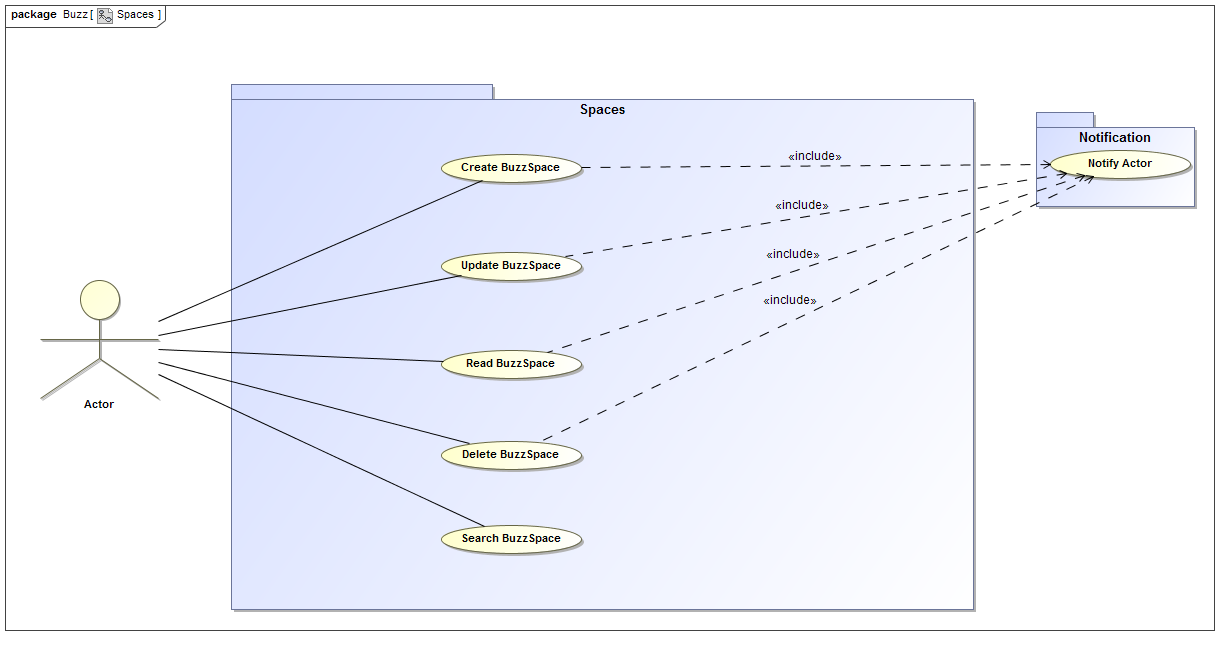
\includegraphics[width=\textwidth]{spacesUseCase}
	\subsection{Short description}
	\begin{description}
		
		\item[] 
			The following section will discuss the functional requirements of the Spaces section of the BuzzSpace program.
		
		\item[] Different actors:
		\begin{itemize}
			\item Administrator: Has system wide permission.
			\item Lecturer: Has full permission for the current BuzzSpace
			\item User: Has permission for the current BuzzSpace according to the users XP. Administrator and Lecturer are included in users as they will be assigned the required XP.   
		\end{itemize}
		
	\end{description}
	
	\subsection{Use case prioritization}
	\begin{description}
		\item[] Critical
		\begin{itemize}
			\item Create BuzzSpace
			\item Delete BuzzSpace
			\item Update BuzzSpace
			\item Read BuzzSpace
		\end{itemize}
		
		\item[] Important
		\begin{itemize}
			\item Search BuzzSpaces
		\end{itemize}
	\end{description}
	
	\subsection{Use cases}
	\newpage
	\begin{table}
		\begin{tabularx}{\textwidth}{|>{\setlength\hsize{0.4\hsize}\setlength\linewidth{\hsize}}X|>{\setlength\hsize{0.5\hsize}\setlength\linewidth{\hsize}}X|>{\setlength\hsize{0.8\hsize}\setlength\linewidth{\hsize}}X|>{\setlength\hsize{0.8\hsize}\setlength\linewidth{\hsize}}X|>{\setlength\hsize{1.1\hsize}\setlength\linewidth{\hsize}}X|}
			\hline
			\multicolumn{5}{|c|}{\textbf{Use cases for Space}}\\
			\hline
			\paragraph{Actor} & \paragraph{Use Case} & \paragraph{Precondition} & \paragraph{Post-condition} & \paragraph{Description} \\
			
			\hline
			\paragraph{User}
			&
			\paragraph{Create BuzzSpace}
			&
			\begin{itemize}
				\item A group must exist
				\item The actor has permission
			\end{itemize} &
			\begin{itemize}
				\item Space created
			\end{itemize} &
			\paragraph{Create a new BuzzSpace (discussion space within group)}
			\\
			\hline
			
			\paragraph{User}
			&
			\paragraph{Delete BuzzSpace}
			&
			\begin{itemize}
				\item The BuzzSpace exists that wants to be removed
				\item The actor has permission
			\end{itemize} &
			\begin{itemize}
				\item BuzzSpace removed from groups
			\end{itemize} &
			\paragraph{Remove a BuzzSpace from groups and notify the users belonging to that group}
			\\
			\hline
			
			\paragraph{User}
			&
			\paragraph{Update BuzzSpace}
			&
			\begin{itemize}
				\item The Space exists that needs to be updated
				\item The actor has permission
			\end{itemize} &
			\begin{itemize}
				\item State of space changed
			\end{itemize} &
			\paragraph{Allow users with permission to update the BuzzSpace}
			\\
			\hline
			
			\paragraph{User}
			&
			\paragraph{Read BuzzSpace}
			&
			\begin{itemize}
				\item The Space exists
				\item The actor has permission
			\end{itemize} &
			\begin{itemize}
				\item BuzzSpace marked read
			\end{itemize} &
			\paragraph{Allow users with permission to read the BuzzSpaces}
			\\
			\hline
			
			\paragraph{User}
			&
			\paragraph{Search BuzzSpaces}
			&
			\begin{itemize}
				\item Must be a registered user
			\end{itemize} &
			\begin{itemize}
				\item Search list created
			\end{itemize} &
			\paragraph{Search the BuzzSpaces in groups}
			\\
			\hline
			
			
		\end{tabularx}
	\end{table}

	\end{document}
	